
\section{Core concepts}
\subsection{Driver distraction and drowsiness: what the system must recognise}

Distraction is commonly divided into three types \cite{r72,r75}. Visual distraction takes the eyes off the road, manual distraction takes a hand off the wheel, and cognitive distraction takes the mind off driving, with phone use being the clearest example as it combines all three. Drowsiness behaves differently, building up gradually, appearing first as yawning and rubbing of the face, then as longer blinks, and finally as micro-sleeps where the eyes remain closed for a second or more.

We chose four visible cues that a camera can capture reliably (Table \ref{tab:ch3-classes} and Figure \ref{fig:ch3-cues}). Yawning and hand-over-mouth, which is usually a covered yawn, are early signs of fatigue. Drinking and phone use are manual and visual distractions, and phone use alone carries an 800 \gls{aed} fine and four black points in the \gls{uae} \cite{r65}. None of these classes depends on where the head points, ensuring that ordinary mirror checks do not trigger alerts. Eye closure is handled separately through a landmark module (Section \ref{sec:ear}).

\begin{table}[htbp]
\centering
\caption{Target classes and what each one indicates}
\label{tab:ch3-classes}
\footnotesize
\setlength{\tabcolsep}{3pt}
\renewcommand{\arraystretch}{1.15}
\begin{tabular}{|p{0.17\linewidth}|p{0.15\linewidth}|p{0.30\linewidth}|p{0.30\linewidth}|}
\hline
\textbf{Class} & \textbf{Group} & \textbf{What it indicates} & \textbf{Why a detector is needed} \\
\hline
Yawning & Drowsiness & Early fatigue, often repeated before micro-sleeps & Mouth shape is clear, but often partly covered \\
\hline
Hand-over-mouth & Drowsiness & A covered yawn or rubbing the face & Hides the mouth landmarks that rule-based methods use \\
\hline
Drinking & Distraction & Manual and visual distraction & Needs the bottle or cup to be seen as an object \\
\hline
Phone use & Distraction & Manual, visual and cognitive distraction & Needs the phone near the ear or in the hand \\
\hline
\end{tabular}
\end{table}

\begin{figure}[htbp]
\centering
\resizebox{\linewidth}{!}{% Figure 1a of our false-alarm paper (rs2): the four target cues on DMD frames and a negative frame.
% All class boxes use solid lines.
\begin{tikzpicture}[font=\footnotesize]
\newcommand{\cuebox}[7]{% node, y0, x0, y1, x1, colour, label  (fractions of the image)
  \draw[#6, line width=1.4pt] ($(#1.south west)!#2!(#1.north west) + (#1.south west)!#3!(#1.south east) - (#1.south west)$) rectangle ($(#1.south west)!#4!(#1.north west) + (#1.south west)!#5!(#1.south east) - (#1.south west)$);
  \node[above right, fill=#6, text=white, inner sep=1.5pt, font=\scriptsize\bfseries] at ($(#1.south west)!#4!(#1.north west) + (#1.south west)!#3!(#1.south east) - (#1.south west)$) {#7};}
\node[inner sep=0pt] (i1) at (0,0) {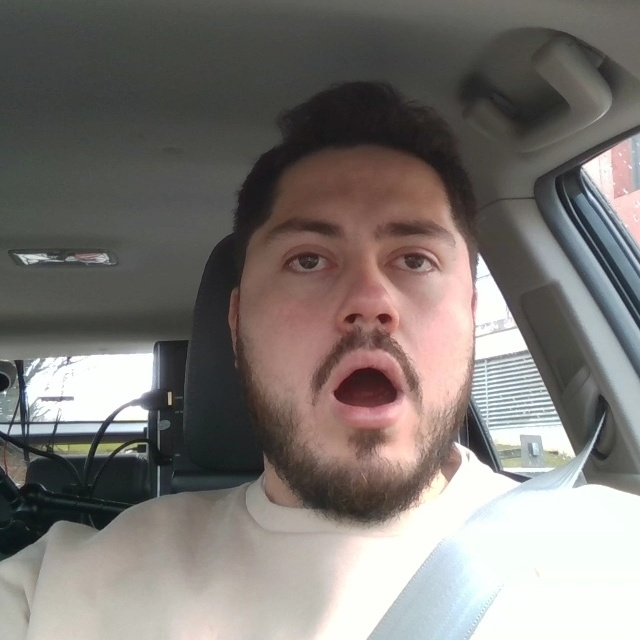
\includegraphics[width=3.0cm, height=3.0cm]{Figures/dmd/cue_yawn.jpg}};
\node[inner sep=0pt, right=0.35cm of i1] (i2) {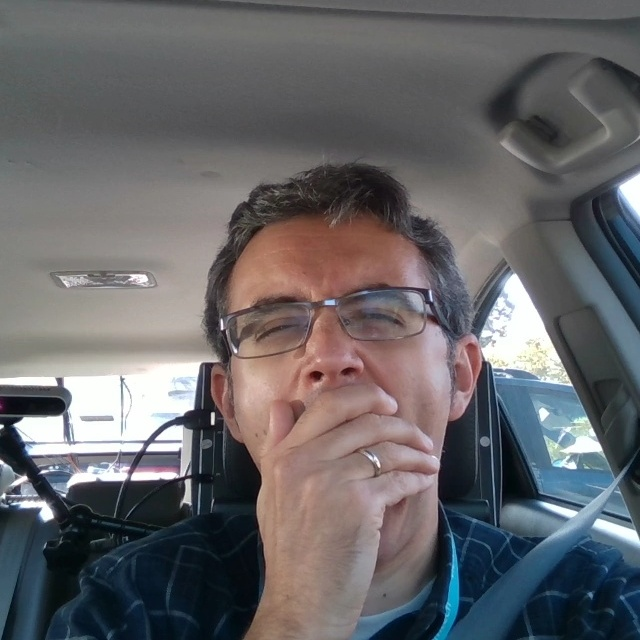
\includegraphics[width=3.0cm, height=3.0cm]{Figures/dmd/cue_hand_mouth.jpg}};
\node[inner sep=0pt, right=0.35cm of i2] (i3) {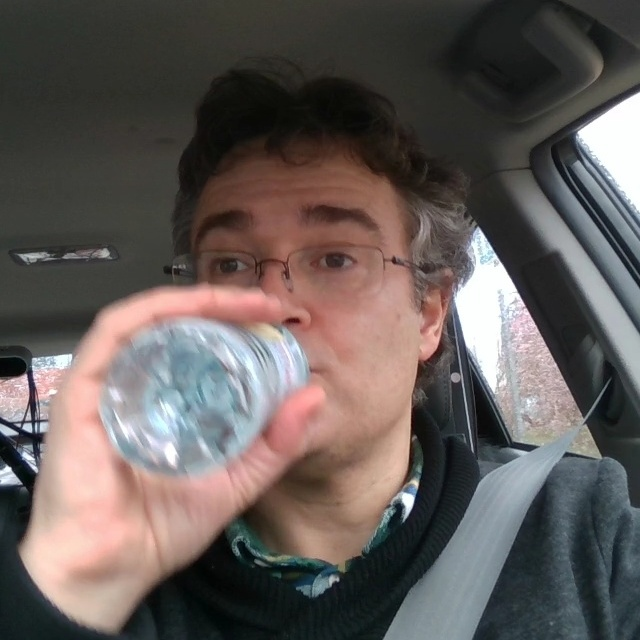
\includegraphics[width=3.0cm, height=3.0cm]{Figures/dmd/cue_drink.jpg}};
\node[inner sep=0pt, right=0.35cm of i3] (i4) {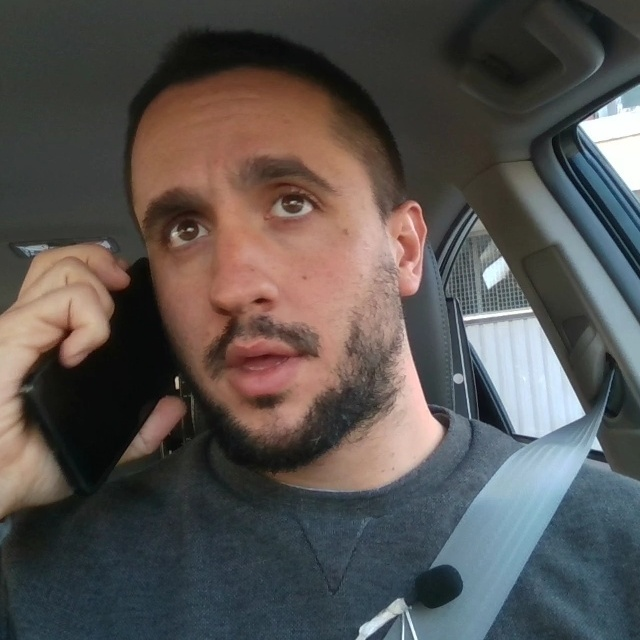
\includegraphics[width=3.0cm, height=3.0cm]{Figures/dmd/cue_phone.jpg}};
\node[inner sep=0pt, right=0.35cm of i4] (i5) {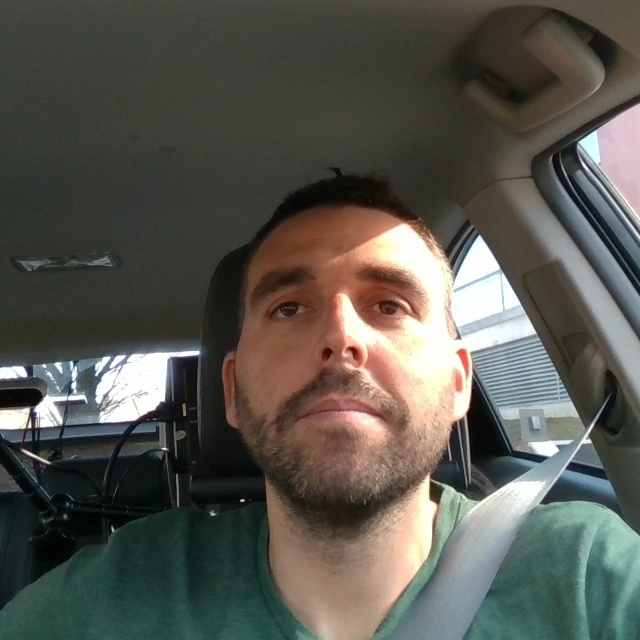
\includegraphics[width=3.0cm, height=3.0cm]{Figures/dmd/cue_negative.jpg}};
\cuebox{i1}{0.32}{0.46}{0.46}{0.67}{red!75!black}{yawn}
\cuebox{i2}{0.05}{0.38}{0.58}{0.70}{cyan!80!black}{hand-mouth}
\cuebox{i3}{0.22}{0.14}{0.56}{0.49}{teal!80!black}{drink}
\cuebox{i4}{0.22}{0.03}{0.63}{0.28}{violet!85!black}{phone}
\node[above left, fill=gray!80!black, text=white, inner sep=2pt, font=\scriptsize\bfseries] at ($(i5.north east) + (-0.08, -0.28)$) {No cue};
\node[below=3pt of i1, font=\small] {Yawning};
\node[below=3pt of i2, font=\small] {Hand-over-mouth};
\node[below=3pt of i3, font=\small] {Drinking};
\node[below=3pt of i4, font=\small] {Phone use};
\node[below=3pt of i5, font=\small] {Negative};
\end{tikzpicture}
}
\caption{The four target classes with their boxes and a negative frame, on DMD frames \cite{r38} (from \cite{rs2}). A covered yawn is labelled hand-over-mouth}
\label{fig:ch3-cues}
\end{figure}

\subsection{Object detection with CNNs and the YOLO family}

A \gls{cnn} learns small filters that slide over an image and respond to edges, textures and shapes. Stacking many of these layers forms a backbone that turns the image into feature maps at several scales. A neck then mixes these scales so that both small objects, such as a phone at the ear, and large ones, such as an open mouth, are represented, and a head predicts a bounding box, a confidence score and a class for every location. Since many neighbouring locations predict the same object, \gls{nms} keeps the highest-scoring box and removes the others that overlap it above an \gls{iou} threshold. A one-stage detector performs all of this in a single pass, which makes it fast enough for video \cite{r44}. Figure \ref{fig:ch3-02} illustrates this structure.

\gls{yolo}11n is the smallest variant of the Ultralytics \gls{yolo}11 family \cite{r45,r46}, with 2.6 million parameters and 6.5 GFLOPs per 640$\times$640 image while reaching 39.5 \gls{map}$_{50-95}$ on \gls{coco}. We rely on transfer learning: the network starts from weights trained on \gls{coco} \cite{r43}, so it already recognises hands, cups and phones, and only needs to learn our four classes from a much smaller dataset.

\begin{figure}[htbp]
\centering
\resizebox{\linewidth}{!}{% How YOLO11n turns one frame into one box, in two rows that read left to right.
\tikzset{ynum/.style={circle, fill=#1, text=white, font=\footnotesize\bfseries, inner sep=1.4pt}}
\begin{tikzpicture}[font=\small, >={Stealth[length=2.6mm]},
  flow/.style={->, line width=1.3pt, gray!70!black},
  title/.style={font=\small\bfseries, align=center},
  note/.style={font=\footnotesize, text=gray!45!black, align=center}]

% ---------------- row 1: input, backbone, neck
\node[inner sep=0pt] (in) at (1.3,0) {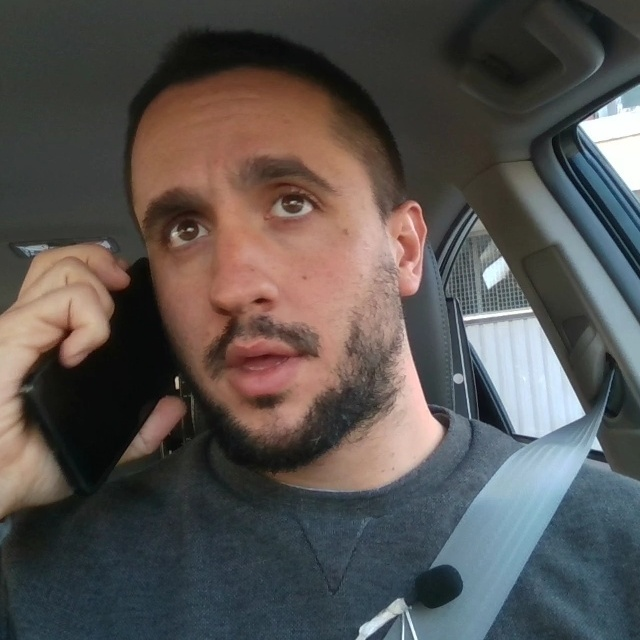
\includegraphics[width=2.6cm]{Figures/dmd/cue_phone.jpg}};
\node[note, below=3pt of in] {640$\times$640 \glsentryshort{roi} crop};
\node[title, above=4pt of in] (tin) {\tikz\node[ynum=gray!70!black]{1};\ Input frame};

\begin{scope}[on background layer]
  \draw[rounded corners=6pt, blue!55!black, fill=blue!3, line width=0.8pt] (3.15,-1.75) rectangle (12.05,1.75);
\end{scope}
\node[title, text=blue!55!black] at (7.6,2.1) {\tikz\node[ynum=blue!55!black]{2};\ Backbone: the image gets smaller, the features get richer};
\foreach \s/\x/\lab in {2.2/3.45/320, 1.8/6.0/160, 1.4/8.2/80, 1.0/9.95/40, 0.6/11.3/20} {
  \pgfmathsetmacro{\st}{\s/4}
  \begin{scope}[shift={(\x,-\s/2)}]
    \draw[fill=blue!13, draw=blue!60!black, line width=0.6pt] (0,0) rectangle (\s,\s);
    \draw[blue!35, step=\st] (0,0) grid (\s,\s);
  \end{scope}
  \node[note] at (\x+\s/2,-1.4) {\lab$\times$\lab};
}
\foreach \a/\b in {5.65/6.0, 7.8/8.2, 9.6/9.95, 10.95/11.3} \draw[->, gray!70!black, line width=0.8pt] (\a,0) -- (\b,0);

\begin{scope}[on background layer]
  \draw[rounded corners=6pt, green!45!black, fill=green!4, line width=0.8pt] (12.75,-1.75) rectangle (16.6,1.75);
\end{scope}
\node[title, text=green!40!black] at (14.7,2.1) {\tikz\node[ynum=green!45!black]{3};\ Neck: mixes the scales};
\foreach \s/\x in {1.2/12.95, 0.9/14.6, 0.6/15.85} {
  \pgfmathsetmacro{\st}{\s/4}
  \begin{scope}[shift={(\x,-\s/2)}]
    \draw[fill=green!15, draw=green!45!black, line width=0.6pt] (0,0) rectangle (\s,\s);
    \draw[green!35!black!40, step=\st] (0,0) grid (\s,\s);
  \end{scope}
}
\draw[<->, green!40!black, line width=0.9pt] (14.15,0) -- (14.6,0);
\draw[<->, green!40!black, line width=0.9pt] (15.5,0) -- (15.85,0);
\node[note] at (14.7,-1.4) {80, 40 and 20 maps};

\draw[flow] (in.east) -- (3.15,0);
\draw[flow] (12.05,0) -- (12.75,0);

% ---------------- row 2: heads, NMS, output
\begin{scope}[on background layer]
  \draw[rounded corners=6pt, red!55!black, fill=red!3, line width=0.8pt] (0,-6.6) rectangle (8.4,-3.6);
\end{scope}
\node[title, text=red!55!black] at (4.2,-7.0) {\tikz\node[ynum=red!55!black]{4};\ Heads: every grid cell guesses a box, a class and a score};
\foreach \x/\g/\what in {1.4/80/small objects, 4.2/40/medium objects, 7.0/20/large objects} {
  \node[draw=red!55!black, fill=red!9, rounded corners=3pt, text width=2.3cm, align=center, minimum height=1.5cm, line width=0.6pt]
    at (\x,-5.1) {\textbf{\g$\times$\g{} grid}\\[1pt]\footnotesize \what};
}
\draw[flow] (14.7,-1.75) -- (14.7,-2.75) -| (4.2,-3.6);

% NMS: many overlapping guesses, one box kept
\node[title, text=orange!70!black] at (11.0,-3.25) {\tikz\node[ynum=orange!75!black]{5};\ \glsentryshort{nms}};
\begin{scope}[shift={(9.9,-5.75)}]
  \draw[gray!60, line width=0.8pt] (0.15,0.25) rectangle (1.75,2.0);
  \draw[gray!60, line width=0.8pt] (0.45,0.05) rectangle (2.05,1.75);
  \draw[gray!60, line width=0.8pt] (0.0,0.0) rectangle (1.6,1.8);
  \draw[orange!85!black, line width=2pt] (0.3,0.15) rectangle (1.9,1.9);
\end{scope}
\node[note, text width=3.4cm] at (11.0,-6.65) {many overlapping guesses, keep only the best one};
\draw[flow] (8.4,-5.1) -- (9.7,-5.1);

\node[inner sep=0pt] (out) at (14.7,-5.1) {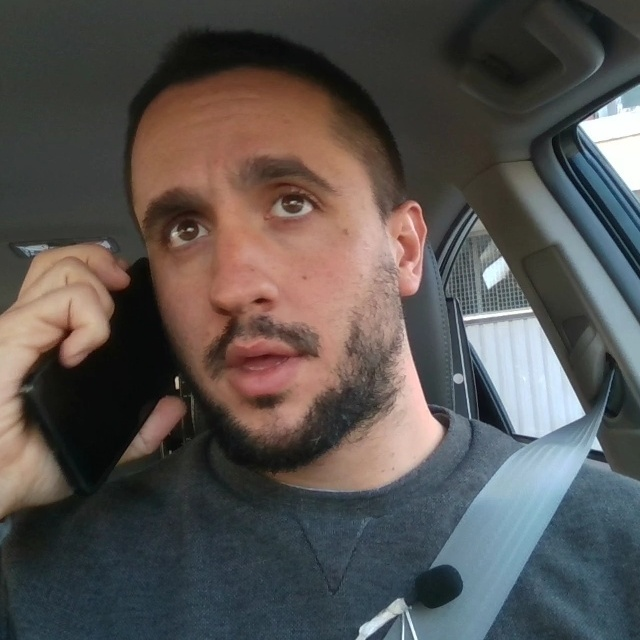
\includegraphics[width=2.6cm]{Figures/dmd/cue_phone.jpg}};
\draw[violet!85!black, line width=1.6pt] ($(out.south west)!0.22!(out.north west) + (out.south west)!0.03!(out.south east) - (out.south west)$) rectangle ($(out.south west)!0.63!(out.north west) + (out.south west)!0.28!(out.south east) - (out.south west)$);
\node[above right, fill=violet!85!black, text=white, inner sep=1.5pt, font=\scriptsize\bfseries] at ($(out.south west)!0.63!(out.north west) + (out.south west)!0.03!(out.south east) - (out.south west)$) {phone};
\node[title, above=4pt of out] {\tikz\node[ynum=violet!85!black]{6};\ Output};
\node[note, below=3pt of out] {one box, class and score};
\draw[flow] (12.25,-5.1) -- (out.west);
\end{tikzpicture}
}
\caption{How \glsentryshort{yolo}11n turns one frame into one box: the backbone shrinks the image into feature maps, the neck mixes fine and coarse maps, three heads guess boxes for small, medium and large objects, and \glsentryshort{nms} keeps the best box}
\label{fig:ch3-02}
\end{figure}

\subsection{Running AI at the edge: Raspberry Pi 5 and the AI HAT+}

The Raspberry Pi 5 has a quad-core Arm Cortex-A76 at 2.4 GHz, two \gls{usb} 3.0 ports and a \gls{pcie} 2.0 $\times$1 lane, and requires a 5 V, 5 A supply \cite{r50}. On the CPU alone, Ultralytics reports \gls{yolo}11n at 6.79 \gls{fps} through \gls{onnx} \cite{r52}, far below our target. The AI HAT+ adds a Hailo \gls{npu} on the \gls{pcie} lane, rated at 13 or 26 \gls{tops} depending on the variant \cite{r51}, running an \gls{int} model compiled with the Hailo toolchain \cite{r70}. Since the \gls{usb} ports are limited to 600 mA on weaker supplies and to 1.6 A with a 5 A supply, power planning matters. Heavy load also heats the board, which throttles above 80--85\,$^\circ$C, making the active cooler a requirement. Processing everything on-device means that raw video never needs to leave the device, and only event records do.

\section{Principles used in the project}
\subsection{Temporal smoothing with an exponential moving average}

A detector scores every frame independently, so a single odd frame can produce a spike. We therefore smooth each class score $x_t$ with an \gls{ema}:
\begin{equation}
s_t = \alpha\,x_t + (1-\alpha)\,s_{t-1}, \qquad \alpha = 1 - e^{-\Delta t/\tau}
\label{eq:ema}
\end{equation}
where $\Delta t$ is the measured time since the last frame and $\tau$ is a time constant in seconds. Defining $\alpha$ through $\Delta t$ ensures the filter forgets at the same rate in seconds whether the pipeline runs at 15 or 30 \gls{fps}, as Figure \ref{fig:ch3-ema-weights} shows. A larger $\tau$ suppresses more noise at the cost of a slower response: for a cue that suddenly appears, the smoothed score crosses a cutoff $\theta$ after
\begin{equation}
t_\theta = -\tau \ln(1-\theta).
\label{eq:delay}
\end{equation}

\begin{figure}[htbp]
\centering
\resizebox{\linewidth}{!}{\begin{tikzpicture}
\begin{axis}[width=15cm, height=6cm, xmin=0, xmax=7, ymin=0, ymax=1.0, xlabel={Time (s)},
  ytick={0,0.5,1}, axis lines=left, axis line style={gray!60}, tick style={gray!60},
  tick label style={font=\small, text=gray}, label style={font=\small, text=gray}, clip=false]
  \addplot[gray!30, line width=0.5pt] coordinates {(0.000,0.111) (0.033,0.000) (0.067,0.063) (0.100,0.033) (0.133,0.036) (0.167,0.044) (0.200,0.000) (0.233,0.043) (0.267,0.024) (0.300,0.150) (0.333,0.057) (0.367,0.039) (0.400,0.042) (0.433,0.030) (0.467,0.018) (0.500,0.038) (0.533,0.064) (0.567,0.043) (0.600,0.079) (0.633,0.044) (0.667,0.051) (0.700,0.096) (0.733,0.066) (0.767,0.035) (0.800,0.900) (0.833,0.066) (0.867,0.108) (0.900,0.042) (0.933,0.043) (0.967,0.080) (1.000,0.023) (1.033,0.041) (1.067,0.076) (1.100,0.067) (1.133,0.053) (1.167,0.070) (1.200,0.000) (1.233,0.081) (1.267,0.021) (1.300,0.000) (1.333,0.058) (1.367,0.071) (1.400,0.037) (1.433,0.018) (1.467,0.051) (1.500,0.048) (1.533,0.092) (1.567,0.072) (1.600,0.900) (1.633,0.083) (1.667,0.044) (1.700,0.022) (1.733,0.068) (1.767,0.067) (1.800,0.044) (1.833,0.027) (1.867,0.057) (1.900,0.000) (1.933,0.071) (1.967,0.065) (2.000,0.001) (2.033,0.052) (2.067,0.021) (2.100,0.073) (2.133,0.000) (2.167,0.023) (2.200,0.071) (2.233,0.085) (2.267,0.000) (2.300,0.035) (2.333,0.060) (2.367,0.032) (2.400,0.098) (2.433,0.014) (2.467,0.061) (2.500,0.019) (2.533,0.092) (2.567,0.049) (2.600,0.039) (2.633,0.000) (2.667,0.100) (2.700,0.073) (2.733,0.073) (2.767,0.084) (2.800,0.060) (2.833,0.031) (2.867,0.026) (2.900,0.026) (2.933,0.091) (2.967,0.006) (3.000,0.847) (3.033,0.809) (3.067,0.868) (3.100,0.822) (3.133,0.841) (3.167,0.852) (3.200,0.843) (3.233,0.841) (3.267,0.808) (3.300,0.841) (3.333,0.743) (3.367,0.842) (3.400,0.790) (3.433,0.906) (3.467,0.913) (3.500,0.752) (3.533,0.857) (3.567,0.844) (3.600,0.798) (3.633,0.877) (3.667,0.827) (3.700,0.762) (3.733,0.837) (3.767,0.843) (3.800,0.855) (3.833,0.788) (3.867,0.881) (3.900,0.887) (3.933,0.793) (3.967,0.817) (4.000,0.846) (4.033,0.822) (4.067,0.937) (4.100,0.860) (4.133,0.799) (4.167,0.811) (4.200,0.847) (4.233,0.965) (4.267,0.841) (4.300,0.856) (4.333,0.876) (4.367,0.848) (4.400,0.964) (4.433,0.823) (4.467,0.887) (4.500,0.858) (4.533,0.881) (4.567,0.791) (4.600,0.938) (4.633,0.844) (4.667,0.852) (4.700,0.803) (4.733,0.814) (4.767,0.878) (4.800,0.899) (4.833,0.888) (4.867,0.910) (4.900,0.886) (4.933,0.851) (4.967,0.892) (5.000,0.880) (5.033,0.845) (5.067,0.886) (5.100,0.914) (5.133,0.862) (5.167,0.832) (5.200,0.027) (5.233,0.036) (5.267,0.025) (5.300,0.040) (5.333,0.076) (5.367,0.038) (5.400,0.045) (5.433,0.074) (5.467,0.069) (5.500,0.101) (5.533,0.000) (5.567,0.076) (5.600,0.036) (5.633,0.054) (5.667,0.075) (5.700,0.082) (5.733,0.081) (5.767,0.055) (5.800,0.098) (5.833,0.042) (5.867,0.046) (5.900,0.074) (5.933,0.033) (5.967,0.115) (6.000,0.081) (6.033,0.115) (6.067,0.049) (6.100,0.039) (6.133,0.055) (6.167,0.072) (6.200,0.032) (6.233,0.061) (6.267,0.049) (6.300,0.098) (6.333,0.030) (6.367,0.081) (6.400,0.031) (6.433,0.021) (6.467,0.029) (6.500,0.014) (6.533,0.054) (6.567,0.081) (6.600,0.055) (6.633,0.069) (6.667,0.099) (6.700,0.058) (6.733,0.056) (6.767,0.042) (6.800,0.002) (6.833,0.073) (6.867,0.000) (6.900,0.070) (6.933,0.050) (6.967,0.084)};
  \addplot[sbblue!45, line width=1.2pt, densely dashed] coordinates {(0.000,0.000) (0.067,0.007) (0.133,0.010) (0.200,0.009) (0.267,0.010) (0.333,0.015) (0.400,0.018) (0.467,0.018) (0.533,0.023) (0.600,0.029) (0.667,0.031) (0.733,0.035) (0.800,0.126) (0.867,0.124) (0.933,0.115) (1.000,0.106) (1.067,0.103) (1.133,0.097) (1.200,0.087) (1.267,0.080) (1.333,0.078) (1.400,0.074) (1.467,0.071) (1.533,0.073) (1.600,0.160) (1.667,0.148) (1.733,0.140) (1.800,0.129) (1.867,0.122) (1.933,0.116) (2.000,0.104) (2.067,0.096) (2.133,0.086) (2.200,0.084) (2.267,0.075) (2.333,0.074) (2.400,0.076) (2.467,0.074) (2.533,0.076) (2.600,0.072) (2.667,0.075) (2.733,0.075) (2.800,0.074) (2.867,0.069) (2.933,0.071) (3.000,0.152) (3.067,0.228) (3.133,0.292) (3.200,0.350) (3.267,0.398) (3.333,0.435) (3.400,0.472) (3.467,0.518) (3.533,0.554) (3.600,0.580) (3.667,0.606) (3.733,0.630) (3.800,0.654) (3.867,0.678) (3.933,0.690) (4.000,0.706) (4.067,0.730) (4.133,0.738) (4.200,0.749) (4.267,0.759) (4.333,0.771) (4.400,0.791) (4.467,0.801) (4.533,0.810) (4.600,0.823) (4.667,0.826) (4.733,0.825) (4.800,0.833) (4.867,0.841) (4.933,0.842) (5.000,0.846) (5.067,0.850) (5.133,0.851) (5.200,0.765) (5.267,0.687) (5.333,0.623) (5.400,0.562) (5.467,0.510) (5.533,0.457) (5.600,0.412) (5.667,0.377) (5.733,0.346) (5.800,0.320) (5.867,0.291) (5.933,0.264) (6.000,0.245) (6.067,0.224) (6.133,0.206) (6.200,0.188) (6.267,0.173) (6.333,0.158) (6.400,0.145) (6.467,0.133) (6.533,0.124) (6.600,0.117) (6.667,0.115) (6.733,0.109) (6.800,0.098) (6.867,0.087) (6.933,0.083)};
  \addplot[sbblue, line width=1.6pt] coordinates {(0.000,0.000) (0.033,0.000) (0.067,0.003) (0.100,0.005) (0.133,0.007) (0.167,0.009) (0.200,0.008) (0.233,0.010) (0.267,0.011) (0.300,0.018) (0.333,0.020) (0.367,0.021) (0.400,0.023) (0.433,0.023) (0.467,0.023) (0.500,0.024) (0.533,0.026) (0.567,0.027) (0.600,0.029) (0.633,0.030) (0.667,0.031) (0.700,0.035) (0.733,0.037) (0.767,0.036) (0.800,0.083) (0.833,0.082) (0.867,0.084) (0.900,0.081) (0.933,0.079) (0.967,0.079) (1.000,0.076) (1.033,0.074) (1.067,0.075) (1.100,0.074) (1.133,0.073) (1.167,0.073) (1.200,0.069) (1.233,0.070) (1.267,0.067) (1.300,0.063) (1.333,0.063) (1.367,0.063) (1.400,0.062) (1.433,0.060) (1.467,0.059) (1.500,0.059) (1.533,0.060) (1.567,0.061) (1.600,0.106) (1.633,0.105) (1.667,0.102) (1.700,0.098) (1.733,0.096) (1.767,0.094) (1.800,0.092) (1.833,0.088) (1.867,0.086) (1.900,0.082) (1.933,0.081) (1.967,0.080) (2.000,0.076) (2.033,0.075) (2.067,0.072) (2.100,0.072) (2.133,0.068) (2.167,0.065) (2.200,0.066) (2.233,0.067) (2.267,0.063) (2.300,0.062) (2.333,0.062) (2.367,0.060) (2.400,0.062) (2.433,0.059) (2.467,0.059) (2.500,0.057) (2.533,0.059) (2.567,0.059) (2.600,0.058) (2.633,0.054) (2.667,0.057) (2.700,0.058) (2.733,0.059) (2.767,0.060) (2.800,0.060) (2.833,0.058) (2.867,0.057) (2.900,0.055) (2.933,0.057) (2.967,0.054) (3.000,0.097) (3.033,0.136) (3.067,0.175) (3.100,0.210) (3.133,0.244) (3.167,0.277) (3.200,0.308) (3.233,0.336) (3.267,0.362) (3.300,0.388) (3.333,0.407) (3.367,0.430) (3.400,0.450) (3.433,0.475) (3.467,0.498) (3.500,0.512) (3.533,0.531) (3.567,0.548) (3.600,0.561) (3.633,0.578) (3.667,0.592) (3.700,0.601) (3.733,0.614) (3.767,0.626) (3.800,0.638) (3.833,0.646) (3.867,0.659) (3.900,0.671) (3.933,0.678) (3.967,0.685) (4.000,0.694) (4.033,0.701) (4.067,0.714) (4.100,0.722) (4.133,0.726) (4.167,0.730) (4.200,0.737) (4.233,0.749) (4.267,0.754) (4.300,0.760) (4.333,0.766) (4.367,0.770) (4.400,0.781) (4.433,0.783) (4.467,0.789) (4.500,0.792) (4.533,0.797) (4.567,0.797) (4.600,0.805) (4.633,0.807) (4.667,0.809) (4.700,0.809) (4.733,0.809) (4.767,0.813) (4.800,0.817) (4.833,0.821) (4.867,0.826) (4.900,0.829) (4.933,0.831) (4.967,0.834) (5.000,0.836) (5.033,0.837) (5.067,0.839) (5.100,0.843) (5.133,0.844) (5.167,0.844) (5.200,0.800) (5.233,0.758) (5.267,0.719) (5.300,0.682) (5.333,0.649) (5.367,0.616) (5.400,0.585) (5.433,0.558) (5.467,0.531) (5.500,0.508) (5.533,0.481) (5.567,0.459) (5.600,0.436) (5.633,0.415) (5.667,0.397) (5.700,0.380) (5.733,0.364) (5.767,0.347) (5.800,0.334) (5.833,0.318) (5.867,0.303) (5.900,0.291) (5.933,0.277) (5.967,0.268) (6.000,0.258) (6.033,0.250) (6.067,0.239) (6.100,0.229) (6.133,0.219) (6.167,0.211) (6.200,0.202) (6.233,0.194) (6.267,0.186) (6.300,0.181) (6.333,0.173) (6.367,0.168) (6.400,0.161) (6.433,0.153) (6.467,0.147) (6.500,0.139) (6.533,0.135) (6.567,0.132) (6.600,0.128) (6.633,0.125) (6.667,0.123) (6.700,0.120) (6.733,0.116) (6.767,0.112) (6.800,0.106) (6.833,0.104) (6.867,0.099) (6.900,0.097) (6.933,0.095) (6.967,0.094)};
  \addplot[sbgold!90!black, line width=1.6pt] coordinates {(0.000,0.006) (0.067,0.009) (0.133,0.011) (0.200,0.010) (0.267,0.011) (0.333,0.013) (0.400,0.015) (0.467,0.015) (0.533,0.018) (0.600,0.021) (0.667,0.023) (0.733,0.025) (0.800,0.072) (0.867,0.074) (0.933,0.072) (1.000,0.070) (1.067,0.070) (1.133,0.069) (1.200,0.065) (1.267,0.063) (1.333,0.063) (1.400,0.061) (1.467,0.061) (1.533,0.063) (1.600,0.108) (1.667,0.104) (1.733,0.102) (1.800,0.099) (1.867,0.097) (1.933,0.095) (2.000,0.090) (2.067,0.087) (2.133,0.082) (2.200,0.081) (2.267,0.077) (2.333,0.076) (2.400,0.077) (2.467,0.076) (2.533,0.077) (2.600,0.075) (2.667,0.076) (2.733,0.076) (2.800,0.075) (2.867,0.073) (2.933,0.074) (3.000,0.115) (3.067,0.156) (3.133,0.193) (3.200,0.228) (3.267,0.260) (3.333,0.286) (3.400,0.313) (3.467,0.345) (3.533,0.373) (3.600,0.396) (3.667,0.419) (3.733,0.442) (3.800,0.464) (3.867,0.487) (3.933,0.503) (4.000,0.522) (4.067,0.544) (4.133,0.558) (4.200,0.574) (4.267,0.588) (4.333,0.604) (4.400,0.623) (4.467,0.637) (4.533,0.651) (4.600,0.666) (4.667,0.676) (4.733,0.684) (4.800,0.695) (4.867,0.707) (4.933,0.715) (5.000,0.724) (5.067,0.732) (5.133,0.739) (5.200,0.701) (5.267,0.664) (5.333,0.633) (5.400,0.601) (5.467,0.572) (5.533,0.541) (5.600,0.514) (5.667,0.490) (5.733,0.468) (5.800,0.448) (5.867,0.426) (5.933,0.405) (6.000,0.388) (6.067,0.369) (6.133,0.352) (6.200,0.335) (6.267,0.320) (6.333,0.304) (6.400,0.289) (6.467,0.275) (6.533,0.263) (6.600,0.252) (6.667,0.244) (6.733,0.233) (6.800,0.221) (6.867,0.209) (6.933,0.200)};
  \draw[sbred, line width=0.6pt] (axis cs:0,0.50) -- (axis cs:7,0.50);
  % direct labels instead of a legend
  \node[anchor=west, font=\small, text=sbred] at (axis cs:7,0.50) {cutoff};
  \node[anchor=south, font=\small, text=gray] at (axis cs:1.2,0.92) {single-frame spikes};
  \node[anchor=west, font=\small, text=sbblue, align=left] at (axis cs:7,0.06) {$\alpha$ from $\Delta t$\\[-2pt]30 and 15 FPS};
  \node[anchor=west, font=\small, text=sbgold!80!black] at (axis cs:7,0.22) {fixed $\alpha$, 15 FPS};
  % the finding
  \draw[{Stealth[length=2mm]}-{Stealth[length=2mm]}, black, line width=0.7pt] (axis cs:3.500,0.36) -- (axis cs:3.933,0.36);
  \node[anchor=north, font=\small] at (axis cs:3.717,0.34) {0.43\,s late};
  \draw[gray!60, densely dotted] (axis cs:3.500,0.36) -- (axis cs:3.500,0.50);
  \draw[gray!60, densely dotted] (axis cs:3.933,0.36) -- (axis cs:3.933,0.50);
\end{axis}
\end{tikzpicture}
}
\caption{The same cue filtered at 30 and 15 \glsentryshort{fps} with $\tau=0.6$\,s: both cross the cutoff at almost the same time, single-frame spikes stay far below it, and a fixed per-frame $\alpha$ reused at 15 \glsentryshort{fps} reacts about 0.43\,s late (illustrative signal)}
\label{fig:ch3-ema-weights}
\end{figure}


\subsection{Model compression: pruning and quantization}

Models can be made smaller and faster in two ways. Structured pruning removes whole filters or channels whose weights contribute little, usually judged by their magnitude \cite{r47}. Unlike removing single weights, this shrinks the actual tensors, so the CPU or \gls{npu} performs less work without special sparse kernels. The model is then fine-tuned again to recover the lost accuracy.

Quantization stores weights and activations with fewer bits. FP16 halves the memory with almost no loss in accuracy, while \gls{int} maps every value to one of 256 levels using a scale $s$ and a zero point $z$, $q=\mathrm{round}(x/s)+z$ \cite{r48}. \gls{ptq} selects $s$ and $z$ from a small calibration set after training, whereas \gls{qat} simulates the rounding during training and usually loses less accuracy. On the Pi, runtimes such as \gls{onnx} Runtime, NCNN \cite{r73} and TFLite run on the CPU, while the Hailo Dataflow Compiler quantizes the model to \gls{int} and compiles it for the \gls{npu} \cite{r70}.


\subsection{Measuring detector performance}

A detection counts as a \gls{tp} when its class is correct and its \gls{iou} with a labelled box is at least 0.5. Otherwise, it is a \gls{fp}, and a missed labelled box is a \gls{fn}. From these counts:
\begin{equation}
P=\frac{TP}{TP+FP},\qquad R=\frac{TP}{TP+FN},\qquad F_1=\frac{2PR}{P+R},\qquad \mathrm{IoU}=\frac{|A\cap B|}{|A\cup B|}.
\end{equation}
\gls{ap} is the area under the precision-recall curve of one class, and \gls{map} averages it over classes, either at an \gls{iou} of 0.5 or across thresholds from 0.5 to 0.95. For the running system, we add throughput in \gls{fps}, end-to-end latency, and the metric that matters most to a driver:
\begin{equation}
\text{False alarms per hour} = \frac{\text{confirmed alerts on clips with no true cue}}{\text{clip duration in hours}}.
\end{equation}


\subsection{Eye-closure measures: EAR and PERCLOS}
\label{sec:ear}

The \gls{ear} of Soukupová and Čech \cite{r35} uses six eye landmarks $p_1$ to $p_6$:
\begin{equation}
\mathrm{EAR} = \frac{\lVert p_2-p_6\rVert + \lVert p_3-p_5\rVert}{2\,\lVert p_1-p_4\rVert}.
\end{equation}
The \gls{ear} stays roughly constant while the eye is open and drops towards zero as it closes. Since eye shape varies between people, a fixed threshold does not suit every driver, so we take each driver's open-eye value from a 20\,s baseline and treat the eye as closed below 50\% of it. The \gls{ear} also drops when a driver looks down, so it cannot be used on its own. \gls{perclos} is the fraction of time the eyes are closed within a sliding window, here 60\,s, and is a validated measure of drowsiness \cite{r69}. Figure \ref{fig:ch3-04} labels the landmarks.

\begin{figure}[htbp]
  \centering
  \begin{subfigure}[b]{0.49\linewidth}\centering
    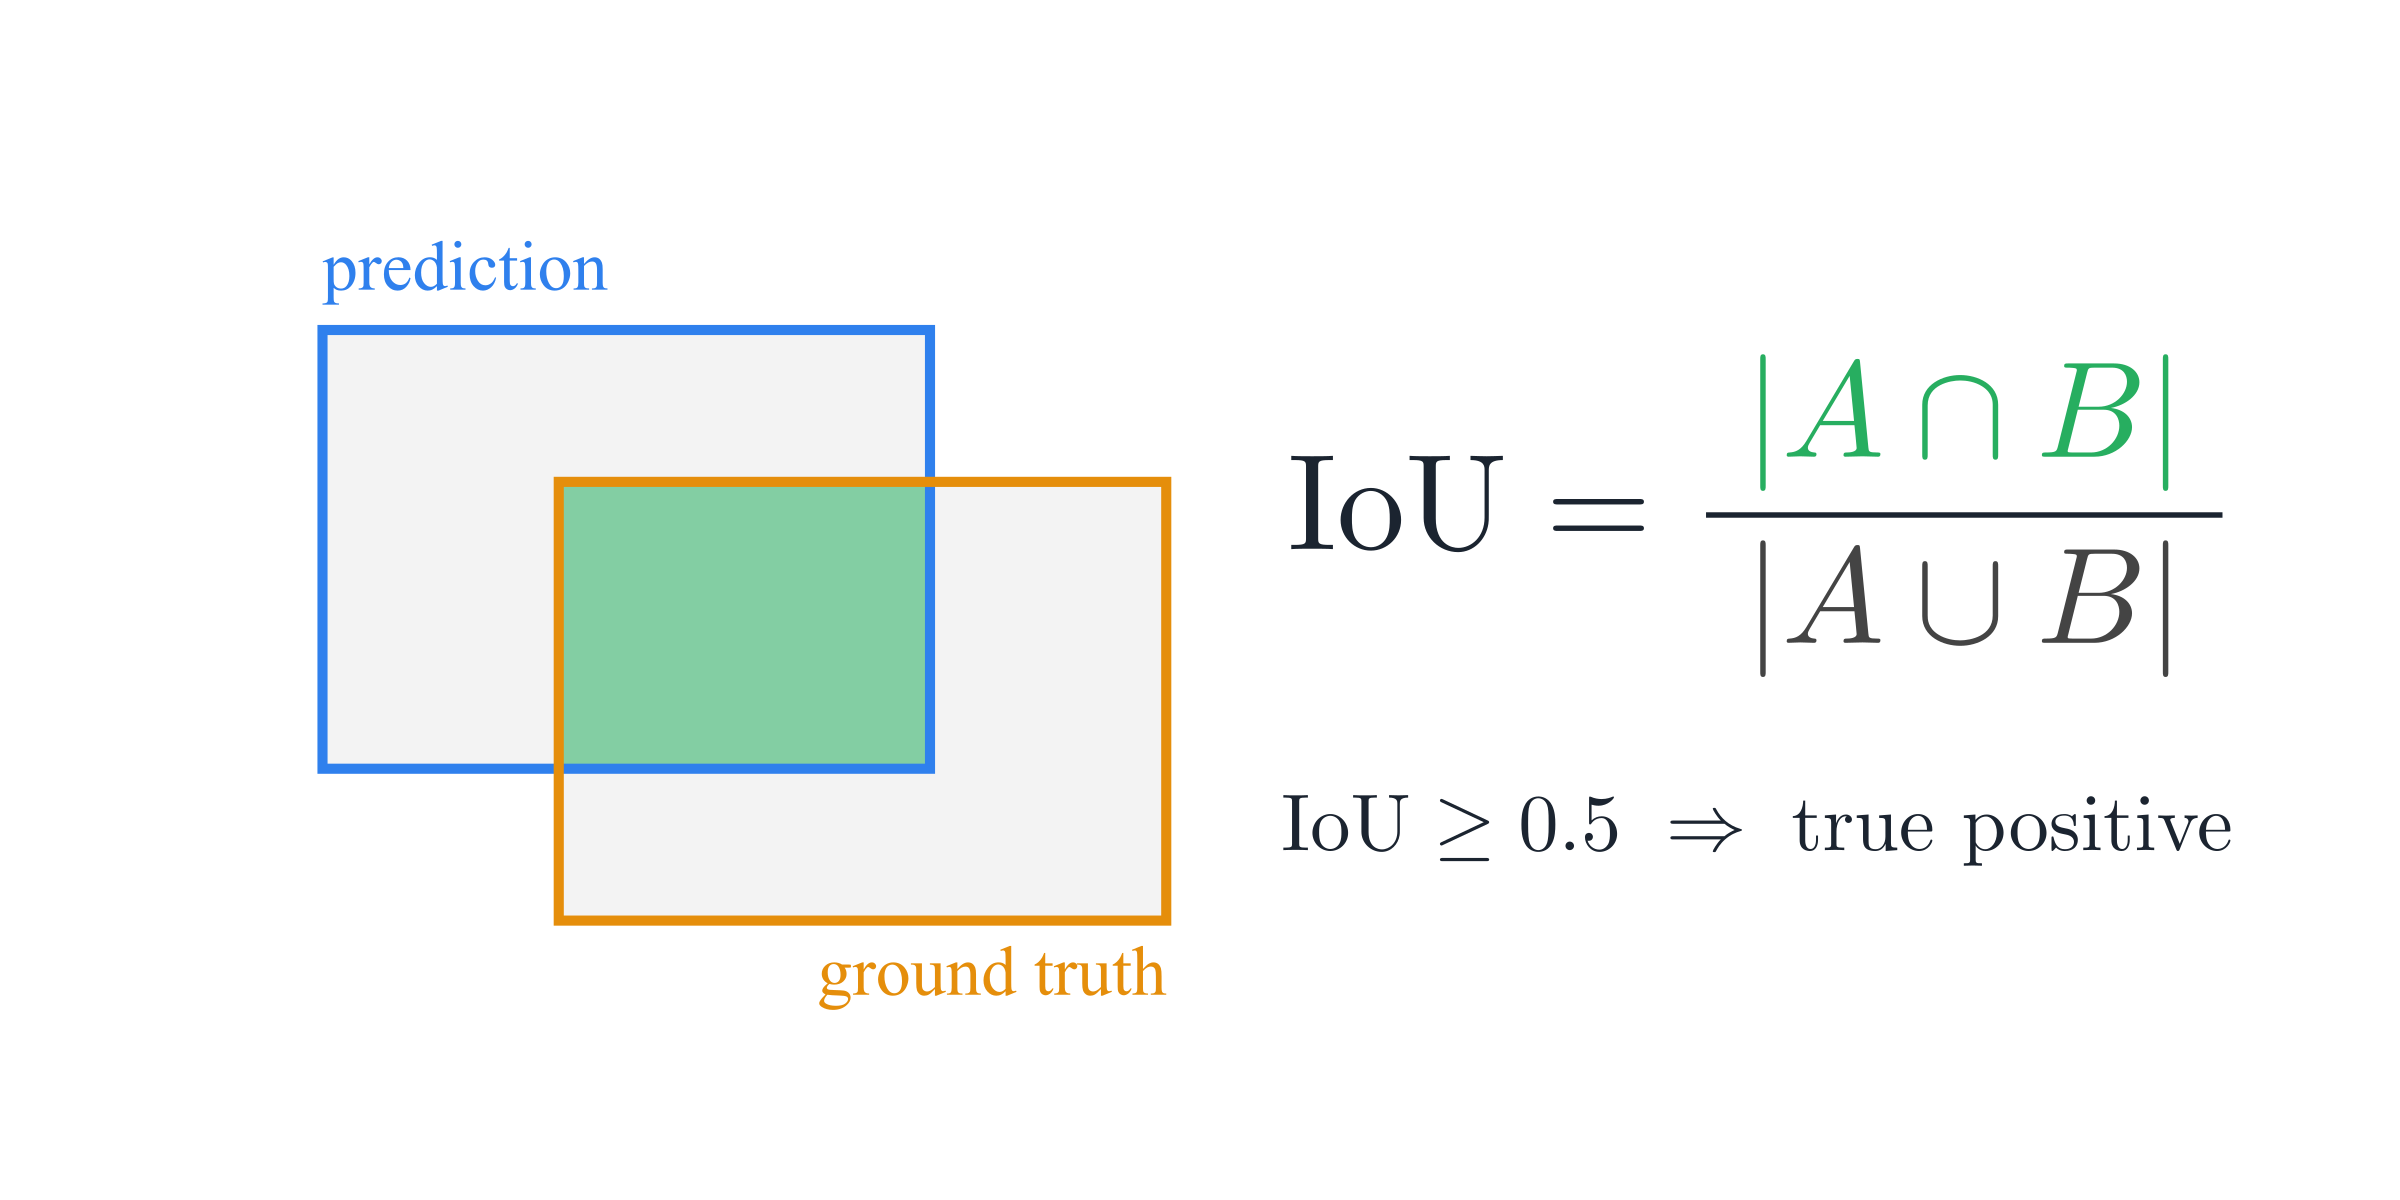
\includegraphics[width=\linewidth]{Figures/eq_IoU.png}
    \caption{\glsentryshort{iou} between a predicted and a ground-truth box}
    \label{fig:ch3-iou}
  \end{subfigure}\hfill
  \begin{subfigure}[b]{0.49\linewidth}\centering
    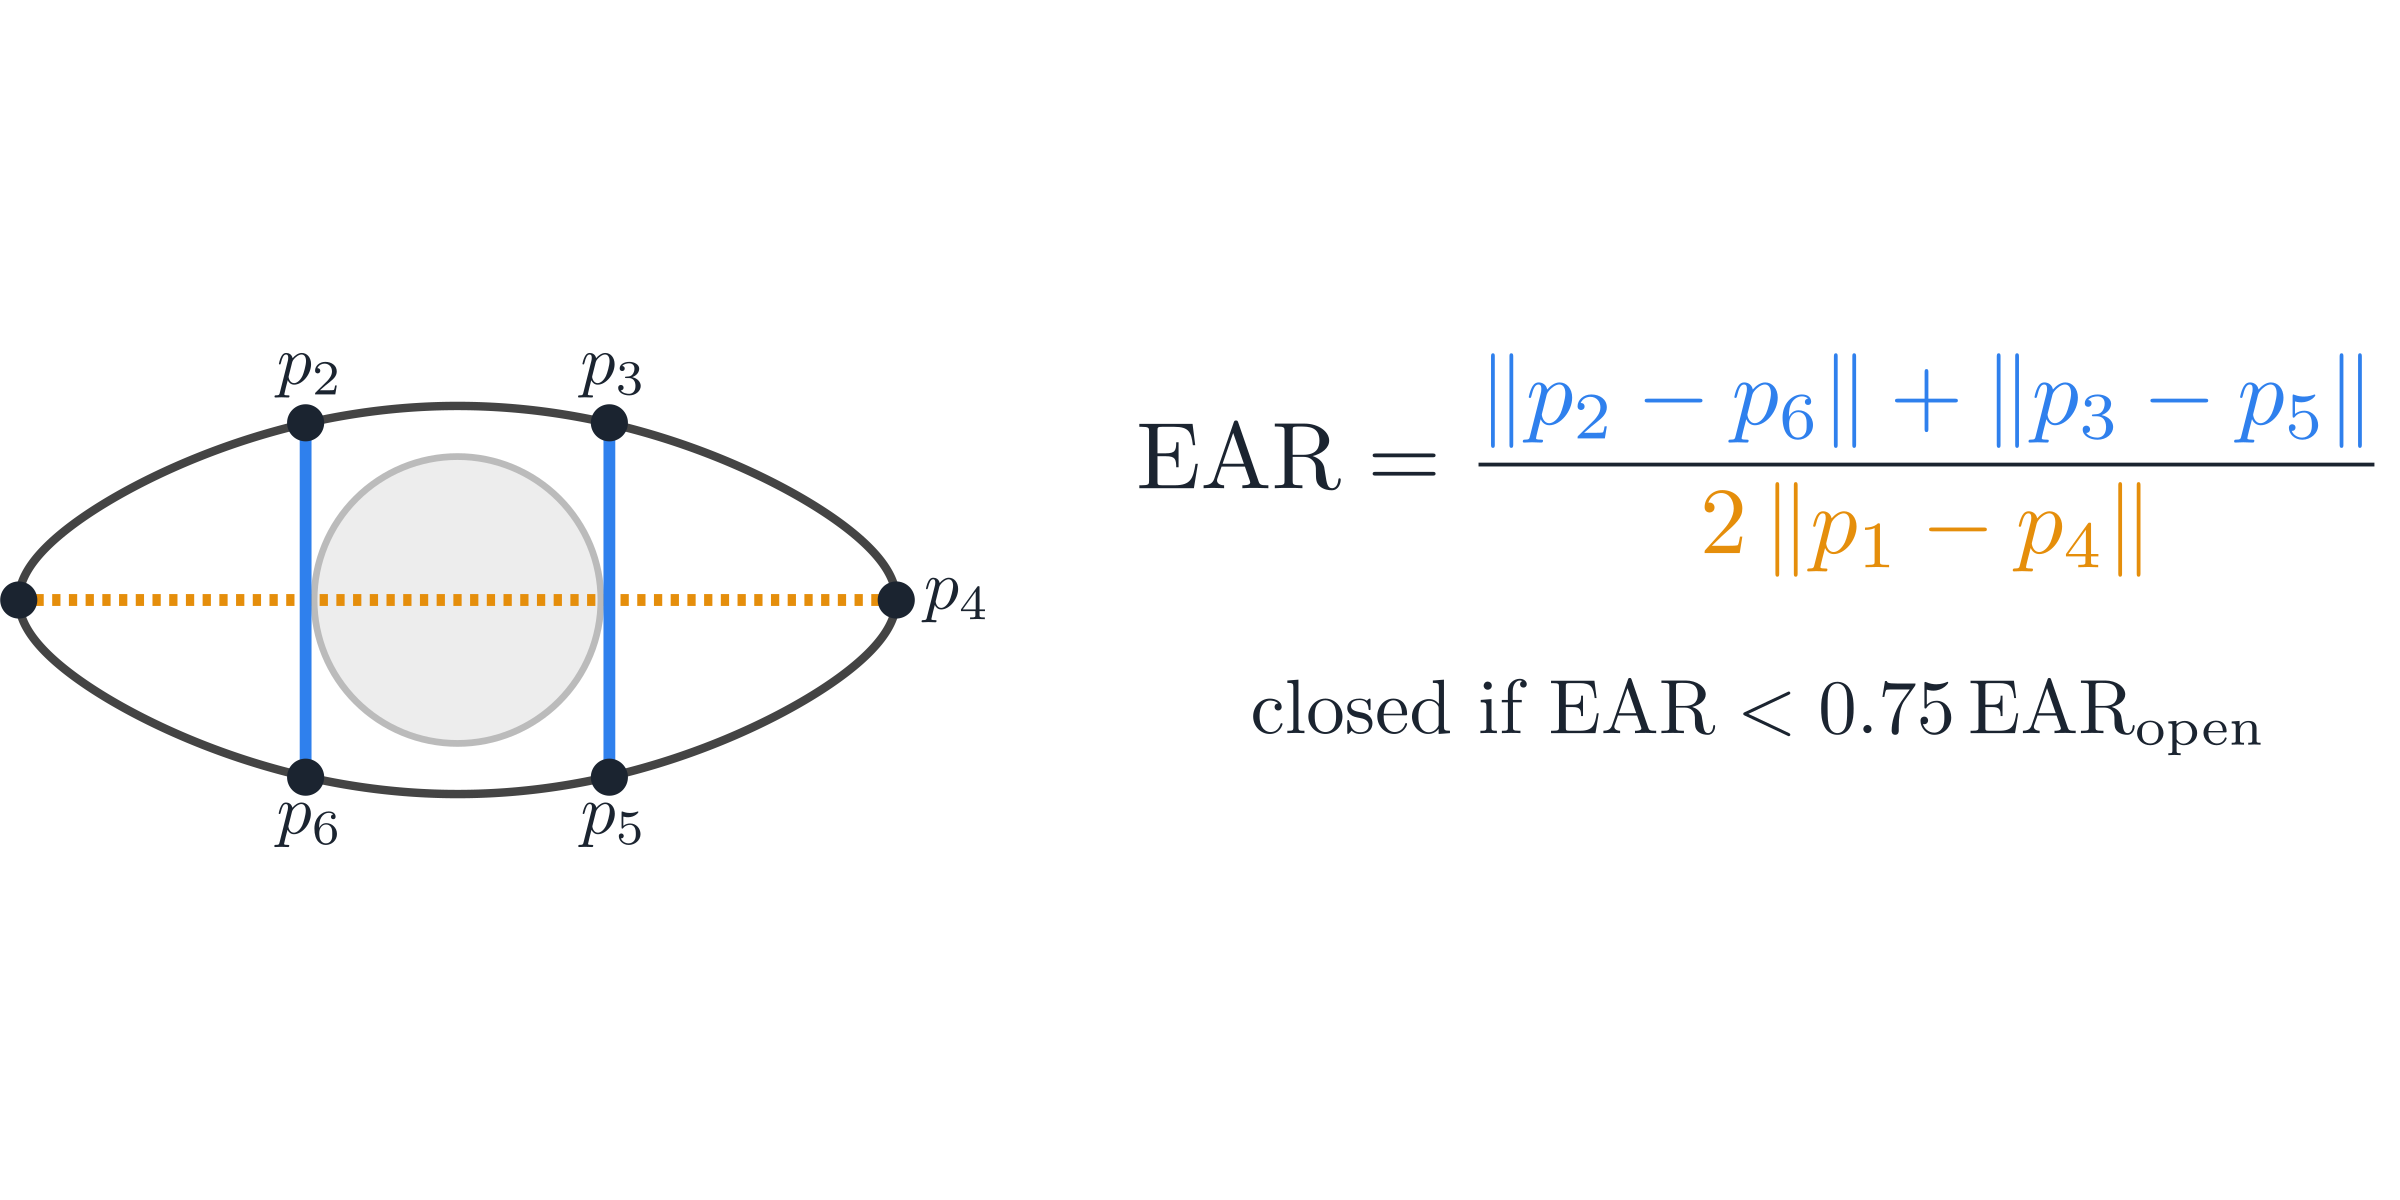
\includegraphics[width=\linewidth]{Figures/eq_EAR.png}
    \caption{Eye landmarks $p_1$--$p_6$ used for the \glsentryshort{ear}}
    \label{fig:ch3-04}
  \end{subfigure}
  \caption{The two geometric measures used in this project}
\end{figure}


\section{Relevant standards, protocols and interfaces}

The system uses common interfaces and follows the standards in Table \ref{tab:ch3-02}.

\begin{table}[htbp]
\centering
\caption{Standards, protocols and how we apply them}
\label{tab:ch3-02}
\footnotesize
\setlength{\tabcolsep}{3pt}
\renewcommand{\arraystretch}{1.15}
\begin{tabular}{|p{0.230\linewidth}|p{0.330\linewidth}|p{0.370\linewidth}|}
\hline
\textbf{Standard / protocol} & \textbf{What it governs} & \textbf{How we apply it} \\
\hline
\gls{usb} / \gls{uvc} \cite{r60} & Plug-and-play video devices & Driverless capture of the C922 through V4L2 \\
\hline
\gls{tls} 1.3 \cite{r54} & Encrypted, authenticated transport & All uploads and map queries use HTTPS \\
\hline
SQLite \gls{wal} \cite{r53} & Crash-safe local database & Event log survives power cuts at ignition-off \\
\hline
\gls{wcag} 2.1, SC 2.3.1 \cite{r55} & No more than three flashes per second & \gls{led} patterns capped at 3 Hz in software \\
\hline
ISO 16750-2 \cite{r58} & Supply voltage ranges in road vehicles & Guides the choice of a future 12 V adapter \\
\hline
ISO 7637-2 \cite{r59} & Transients on vehicle supply lines & Adapter must tolerate cranking dips and load dumps \\
\hline
\gls{uae} \gls{pdpl} \cite{r56} & Processing of personal data in the \gls{uae} & Consent, data minimisation, no video upload \\
\hline
\gls{gdpr} \cite{r57} & Data protection reference & Right to withdraw and delete dataset records \\
\hline
OpenStreetMap Overpass \cite{r68} & Points of interest query & Nearest rest stop or fuel station (Desired) \\
\hline
\end{tabular}
\end{table}
